\lab{Parallel Computing with $\texttt{ipyparallel}$}{Parallel Computing with $\texttt{ipyparallel}$}
\objective{(TODO: Awesome objective coming!)}
\label{lab:parallel1}

\section*{Why Parallel Computing?}
When a single processor takes too long to perform a computationally intensive task, there are two simple solutions.
The first is simply to build a faster processor.
Unfortunately, physics gets in the way.
In particular, the problem of heat dissipation has kept processor speeds from increasing as quickly in recent years as they did in the past.
The second solution is to have mutiple processors work together on the same task.
This is the main idea behind parallel computing. Essentially, a `supercomputer' is made up of many normal computers, each with its own memory.

Today, high computing performance is achieved using many processors.
These processors communicate with each other and coordinate their tasks with a message passing system. The details of this message passing system, MPI, will be the topic of the next lab.

In this lab, we will become familiar with some of the basic ideas behind parallel computing.

\section*{Serial Execution vs. Parallel Execution}
Up to this point, all the programs you have written run in \emph{serial}. This means that each command is executed one line at a time. The following exercise will help you visualize what is happening.

\begin{info}
Engaged Learning Section! Try this out!

If you are working on a Linux computer, open a terminal and execute the \li{htop} command. (If \li{htop} is not on your system, install it using your default package manager). When opening this program, your terminal should see an interface similar to Figure \ref{fig:htop}. The numbered bars at the top represent each of the cores of your processor and the workload on each of these cores.

Now, run the following python code with your terminal running \li{htop} still visible. The sole purpose of the following code is to create a computationally intensive function that runs for about 15 seconds.

\begin{lstlisting}
import numpy as np
for i xrange(10000):
    np.random.random(100000)
\end{lstlisting}

You should have seen one of the cores get maxed out at 100\%. It is also possible that you saw the load-carrying core switch midway through the execution of the file. This is evidence one indicator that our script is being executed in serial -- one line at a time, one core at a time.
\end{info}

\begin{figure}
    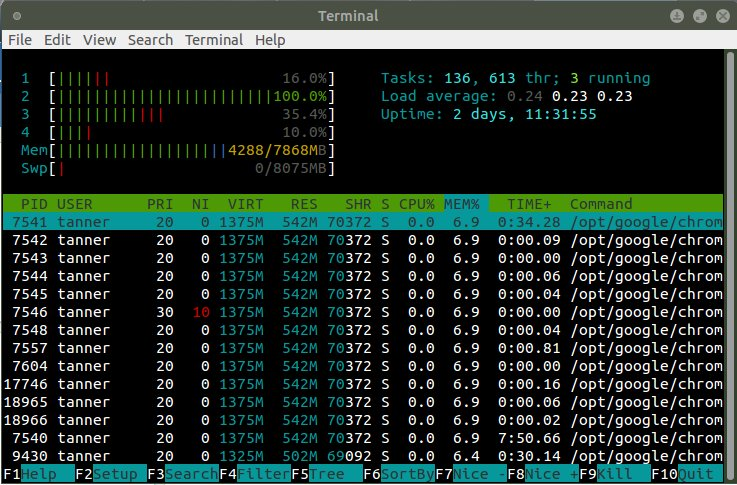
\includegraphics[width=\textwidth]{active.jpg}
\caption{An example of \li{htop} with a computationally intense python script running.}
\label{fig:htop}
\end{figure}

As you saw in the exercise above, only one of the cores was carrying the load at a time. This means that we are only using a fraction of the computer's resources. When working on a personal computer, this would often be to your benefit. Dividing jobs among multiple cores is part of what makes smooth multitasking possible. However, in the event you wish to devote all the computer's resources to executing your code, we employ the help of the \li{ipyparallel} module. In theory, you can make your code run $N$ times faster when executing in parallel where $N$ is the number of cores

\section*{The $\texttt{ipyparallel}$ Module}
We will begin our discussion on parallel computing by learning about the \li{ipyparallel} module. Even though this may not be the fastest parallel computing framework available, it is very easy to take advantage of all the cores on your computer with relatively little code. As mentioned before, you cannot expect your code to magically run faster if you requests the usage of more cores on your computer. You have to specify what happens on each core. This concept is key to understanding parallel computing.

\subsection*{Installation and Initialization of $\texttt{ipyparallel}$}

If you have not already installed \li{ipyparallel}, you may do so using the conda package manager.

\begin{lstlisting}
$ conda update conda
$ conda update anaconda
$ conda install ipyparallel
\end{lstlisting}

TODO Starting up ipcluster.
TODO add a note about enabling the notebook extension
